\section{Einleitung} 

% Die Verlässlichkeit von Web-Anwendungen hat in der heutigen Zeit eine so hohe Relevanz wie noch
% nie zuvor und die Wirtschaftlichkeit von Dienstleistenden IT-Unternehmen hängt stark von der Qualität ihrer Software ab.
% Ein wichtiger Aspekt in Bezug auf die Verlässlichkeit von Software sind Typsysteme, mit ihrem Versprechen eine Vielzahl
% von Fehlern auszuschließen, bevor die Software überhaupt läuft.

Typensicherheit ist ein oft diskutiertes Thema in der Softwareentwicklung. 
Viele Sprachen 

Die folgende Arbeit richtet sich an angehende Softwarearchitekten und soll dabei helfen API-Design sowie Implementation
mithilfe von Typsystemen zu erläutern.
Das Thema wird im folgenden durch anschauliche Beispiele im Kontext von reelen Szenarien praxisnah dargestellt.

\subsection{Grundlagen}

Für das Verständnis der Arbeit wird angenommen,
dass Leser*innen ein Grundlegendes Wissen über Webanwendungen sowie REST-APIs besitzen.
Es ist desweiteren hilfreich, wenn Kenntnisse über TypeScript und JSON vorliegen.
Auch wenn die Typentheorie nicht bekannt sein muss, und alles was in diesem Bezug relevant ist im 
Laufe der Arbeit erläutert wird, sollte ein Basiswissen über die Mengenlehre vorliegen.

% TODO

\subsection{Problemstellung}

Fehler in der Softwareentwicklung sind auch heutzutage noch sehr präsent. Ob in einem Studienprojekt, der Website einer Behörde,
oder dem Betriebssystem eines Millardenkonzerns: Im Alltag trifft man nicht selten auf solche Fehler.

\begin{figure}[H]
  \centering
  \begin{subfigure}[b]{0.4\linewidth}
    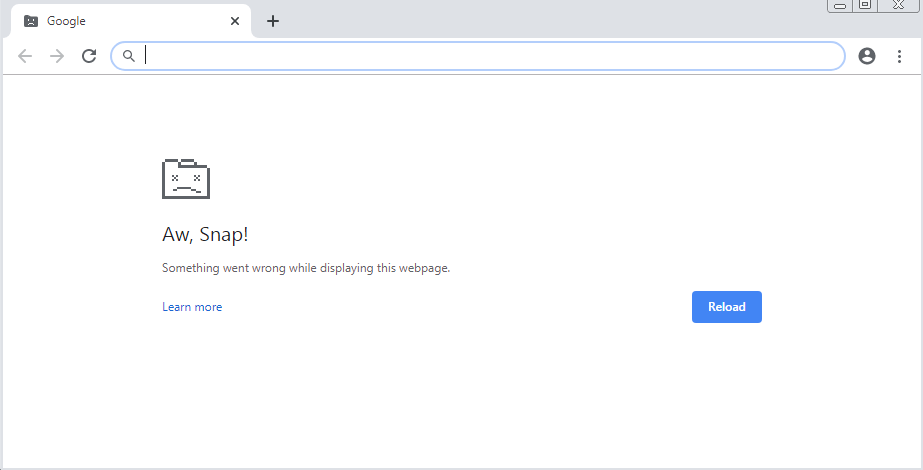
\includegraphics[width=\textwidth]{chrome_error}
    \caption{Ein Crash im Chrome-Browser}
  \end{subfigure}
  \hspace{0.5cm}
  \begin{subfigure}[b]{0.4\linewidth}
    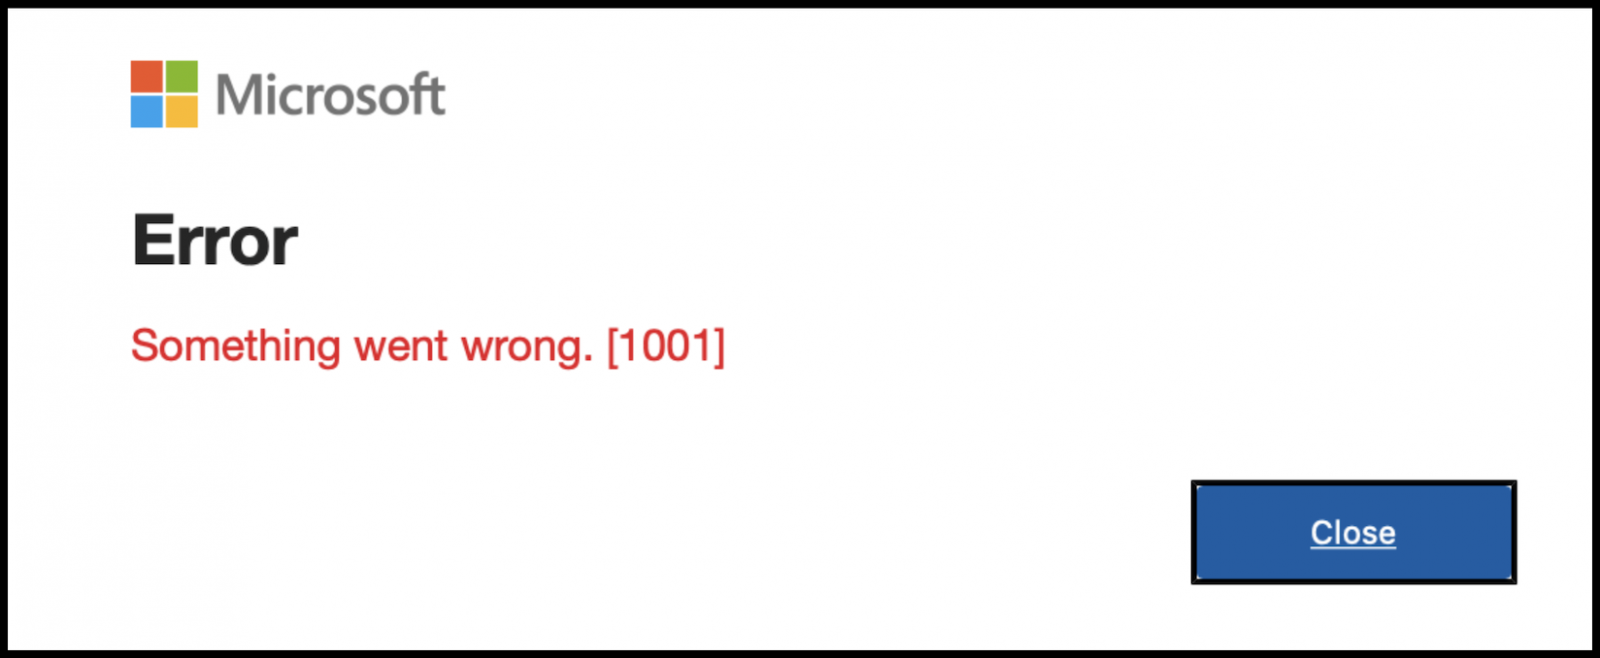
\includegraphics[width=\textwidth]{microsoft_error}
    \caption{Ein Fehler während des Microsoft Logins}
  \end{subfigure}
  \caption{Fehler in alltäglichen Anwendungen}
\end{figure}

Ein Ansatz um Fehler zur Laufzeit von Software zu verhindern sind Typsysteme, wie Beispielsweise von TypeScript welches versucht JavaScript zu typisieren.

\begin{figure}[H]
  \centering
  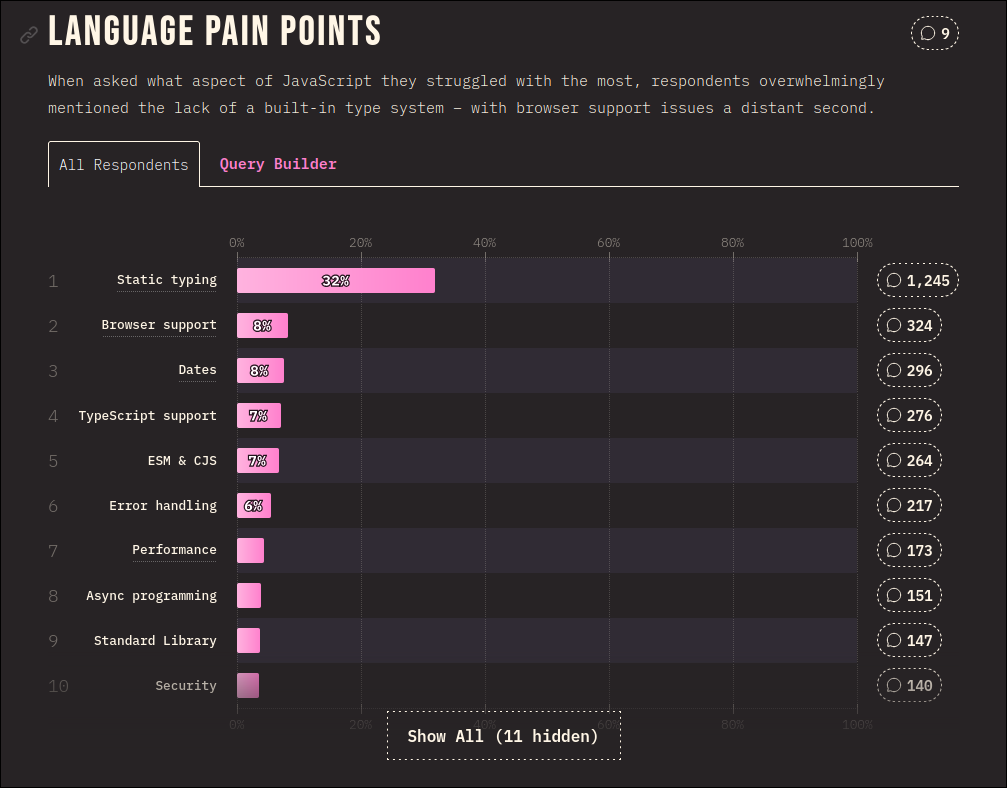
\includegraphics[width=0.9\textwidth]{state_of_js}
  \caption{32\% der Befragten in der \textquote{State of JavaScript 2024} Umfrage gaben an das (fehlende) statische Typisierung einer ihrer größten Probleme mit der Sprache sei \cite{Greif_Burel_2024}}
\end{figure}

Während TypeScript es schafft die Sprache ansich zu typisieren, gibt es in Probleme, sobald Daten zwischen Prozessen
kommuniziert werden sollen.
In modernen Softwarearchitekturen kommunizieren Anwendungen häufig über APIs.
Dabei werden die Datenstrukturen von Anfrage- und Antwort Daten oft mehrfach und in verschiedenen Systemen definiert
- zum Beispiel getrennt im Front- und Backend.
Diese Redundanz führt zu erhöhtem Wartungsaufwand und einem hohen Risiko von Fehlern,
wenn sich Schnittstellen ändern, aber nicht von allen Konsumenten gleichermaßen angepasst werden.

\subsection{Ziel der Arbeit}

In der folgenden Ausarbeitung sollen zunächst Möglichkeiten aufgezeigt werden, wie Schnittstellen Typsicher definiert werden können.
Daraufhin werden Tools präsentiert mit denen Schnittstellen über Systeme hinweg konsistent dargestellt werden können um hohe Wartungsaufwände und Fehler bei Änderungen zu vermeiden.

Insgesamt soll die Arbeit Architekten von Webanwendungen dabei helfen API-Schnittstellen zu definieren und die in der Arbeit erwähnten Tools sinnvoll einzusetzen,
um konsistente, klar definierte und typsichere Endpunkte zu schreiben.
